\chapter{Step 1: Model Specification}\label{dev-step1}

\begin{abstract}
    The model specification stage is common across the three methods identified for comparison. It involves using an XLRM structure to develop a model or models of the system under consideration. There are details of each of the policy structure alternatives identified that will lead to unique XLRM structures for each of the three versions of the lake problem. The specification will explain the model specification in the following order: exogenous uncertainties (\cref{step1-X}), decision levers (\cref{step1-L}), outcomes of interest (\cref{step1-M}), and relations (\cref{step1-R}), or XLMR. This is different from the commonly written order of XLRM, but is done for clarity and to ensure that each component of the model is specified before their relations are described. 
\end{abstract}

\medskip

\begin{figure}[h]
    \centering
    \captionsetup{justification=centering}
    
    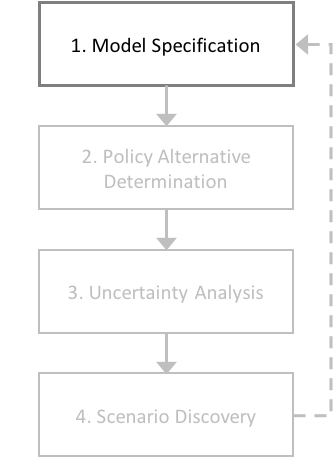
\includegraphics{structure-step1}
    \caption{RDM Structure - Step 1}
    \label{fig:structure-step1}
\end{figure}

\newpage

\section{General Approach}
The first step to each of the identified robust decision support methods is problem specification. This involves building a computer-based model of the problem identified by decision makers. Model development for the three methods compared in this study require an XLRM-based specification structure. The XLRM structure requires the identification of inputs, through uncontrollable uncertainties (X) and adjustable decision levers (L), outcomes of interest or performance measures (M), and relations (R) that describe how different combinations of input values lead to different potential future states of the system under consideration. 

Without an existing well-structured definition of a problem, the XLRM specification is developed through review of the relevant background information and existing literature. The analyst uses that information in combination with conversations among a variety of decision makers and subject-matter experts to ensure that all relevant data and views are incorporated into the defined system \citep{Lempert2003}. In addition to identifying the structure of the problem under consideration, the specification must operationalize decision levers and uncertainty parameters through identifying value ranges, probability distributions, or other means. 

Through research and discussion, a specification of the problem at hand will be developed, which will be used to determine a set of potentially robust policy alternatives. 

\section{The Lake Problem}
For the purposes of this study, a well-researched, well-defined and commonly referenced highly-stylized policy problem is used known as the lake problem. Using an existing well-defined and accepted policy problem allows the focus of the comparison to remain on the two factors under consideration: the impact of the robust decision support method and of the policy implementation structure. 

As such, literature that has previously defined and tested the specification and implementation of this problem is leveraged to build the specification of the lake problem for this study. This section will describe the details following the XLRM structure defined for all three methods of robust decision support. 

    \subsection{"X": Exogenous Uncertainties}\label{step1-X}
    There are five sources of uncertainty in the definition of the lake problem used for this study. The uncertainty ranges and base values have been selected based on the most commonly used settings in literature \citep{Carpenter1999,Eker2018,Hadka2015,Quinn2017,Ward2015}. The specific settings for each uncertainty parameter are found in \cref{table:uncertainties}. 

    \begin{table}[ht]
        \caption{Exogenous uncertainty settings}
        
        \label{table:uncertainties}
        
        \setlength\arrayrulewidth{1pt}\arrayrulecolor{white}
        \rowcolors{2}{odd-row-blue}{even-row-blue}
        \begin{tabularx}{\linewidth}{l|X|l|l}
            \rowcolor{tudelft-dark-blue!80}
            \color{white}\bfseries Name     &      \color{white}\bfseries Description   &
            \color{white}\bfseries Range    &      \color{white}\bfseries Baseline\\ \hline
            
            b               & Pollution rate of removal through natural outflows        & [0.1, 0.45]       & 0.42\\ \hline
            q               & Pollution recycling rate through natural processes        & [2.0, 4.5]        & 2.0\\ \hline
            $\mu$           & Mean of natural pollution inflows                         & [0.01, 0.05]      & 0.02\\ \hline
            $\sigma$        & Standard deviation of natural inflows                     & [0.001, 0.005]    & 0.0017\\ \hline
            $\delta$        & Utility discount factor                                   & [0.93, 0.99]      & 0.98\\
            
        \end{tabularx}
    \end{table}
    
    \subsection{"L": Decision Levers}\label{step1-L}
    The distinguishing piece of the three lake model variations, the decision levers and their implementations. are unique to each model variation. 

        \subsubsection{Intertemporal}
        The intertemporal variation of the lake model, as described in \cref{review-structure}, is defined by a series of independent and static decision levers equal to the number of steps in the time horizon of analysis. Each decision lever, $X_{i}$, with a value in the range of $[0, 0.1]$, specifies the amount of pollution that is released in that time step. 

        \subsubsection{Direct policy search (DPS)}
        The direct policy search variation of the lake problem aims to develop a rule for pollution release that is responsive to the current condition of the lake. This rule is developed using five decision levers, which are described in \cref{table:levers-dps}. These five decision levers combine with the level of pollution in the lake at the previous time step, $X_{t}$, to form a pollution release rule. In this research, as in previous research that concerns DPS policy structures, the release rule takes the form of a cubic radial function, described in \cref{eq:dps-rule}. In the DPS variation of the lake problem, the amount of pollution to release is updated at every step in the time horizon, and so unlike the intertemporal form of the lake model, the DPS variation is able to react to changes in pollution level in real time.

        \begin{equation}\label{eq:dps-rule}
        X_{t} = \begin{cases}
                    0.01 & \alpha < 0.01 \\
                    \alpha & 0.01 <= \alpha <= 0.1 \\
                    0.1 & \alpha > 0.1
                \end{cases}, 
                \text{where } \alpha = w_{1}*(\frac{(X_{t-1}-c_{1})}{r_{1}})^{3} + (1-w_{1})*(\frac{(X_{t-1}-c_{2})}{r_{2}})^{3}
        \end{equation}

        \begin{table}[h]
            %    \centering
            %    \captionsetup{justification=centering}
            \caption{Direct Policy Search Levers}
            
            \label{table:levers-dps}
            
            \setlength\arrayrulewidth{1pt}\arrayrulecolor{white}
            \rowcolors{2}{odd-row-blue}{even-row-blue}
            \begin{tabularx}{\textwidth}{l|X|l|l}
                \rowcolor{tudelft-dark-blue!80}
                \color{white}\bfseries Name     &      \color{white}\bfseries Description   &
                \color{white}\bfseries Range    \\
                
                \hline
                $c_{1}$          & Represents the center of the radial cubic function         & [-2, 2]       \\
                \hline
                $c_{2}$          & Represents the center of the radial cubic function         & [-2, 2]       \\
                \hline
                $r_{1}$          & Represents the radius of the radial cubic function         & [0, 2]        \\
                \hline
                $r_{2}$          & Represents the radius of the radial cubic function         & [0, 2]        \\
                \hline
                $w_{1}$          & The weight of the radial cubic function                    & [0, 1]        \\
                
            \end{tabularx}
        \end{table}

        \subsubsection{Planned adaptive DPS}
        Planned adaptive direct policy search is a proposed new variation of the lake problem that attempts to match policy behavior that is closer to real-world implementations. The fundamental structure of the decision levers match that of the DPS variation, with the same five levers used and following the same function as specified in \cref{eq:dps-rule}. However, instead of updating the amount of pollution released at every time step, the pollution release level is updated every 10 time steps. The slower update of the pollution level is intended to more closely match the fact that decisions like changing the pollution release level takes time to enact and will more than likely not reset after each time step, especially if that time step represents just a year of real-world time, as is the case in the current design of the lake problem \citep{Ward2015}. 

    \subsection{"M": Outcomes of Interest}\label{step1-M}
    The outcomes of interest are common across model variations. Functional definitions can be found in \cref{step0-robust}, but \cref{table:outcomes} describes the outcomes, the value that is returned from a single run of the lake problem, and whether the goal of the outcome is to minimize or maximize the value that is returned. These details, too, were taken from previous literature that has used the lake problem \citep{Quinn2017, Ward2015}. 

    \begin{table}[h]
    %    \centering
        %    \captionsetup{justification=centering}
        \caption{Outcomes of interest}
        
        \label{table:outcomes}
        
        \setlength\arrayrulewidth{1pt}\arrayrulecolor{white}
        \rowcolors{2}{odd-row-blue}{even-row-blue}
        \begin{tabularx}{\linewidth}{|\OutA|\OutB|\OutC|\OutD|}
            \rowcolor{tudelft-dark-blue!80}
            \color{white}\bfseries Name              &      \color{white}\bfseries Description   &
            \color{white}\bfseries Value Returned    &      \color{white}\bfseries Min/ Max       \\
            
            \hline
            Pollution Level   & A measure that tracks the pollution \newline levels in the lake.
                              & Maximum value over time  & Min     \\
            \hline
            Utility           & The economic benefits for the town's agriculture and industry. It is assumed that utility is uniformly discounted over time. 
                              & Mean value over time     & Max     \\
            \hline
            Inertia           & Indicates the stability of the pollution release level over time. 
                              & Mean value over time     & Max     \\
            \hline
            Reliability       & An indication of the percentage of time spent under the critical pollution threshold over time.
                              & Mean value over time     & Max    \\
            
        \end{tabularx}
    \end{table}

    \subsection{"R": Relations}\label{step1-R}
    Every exogenous uncertainty, decision lever, and outcome of interest in each variation of the lake problem is tied together through sets of relations. Additional parameters that are common amongst all three variations of the lake model and that tie these elements together are described in \cref{table:lakeadditional}. These relations are implemented using the Cython optimizing compiler for Python. By developing each lake model in Cython, the analysis will be able to reduce the time required for computation of model-specific values. The code used is based off of the lake model as designed for the EMA-Workbench, a python-based open-sourced toolkit that supports multi-objective optimization, uncertainty analysis, and scenario discovery \citep{Kwakkel2017}. The EMA-Workbench toolkit will be used throughout the analysis steps, along with the Platypus optimization library, which will provide the required optimization functionality. 
    
    Additional common properties tying these elements together are the length of the time horizon considered, which is set to 100 steps, and the number of repetitions for which each lake model will be run for a single experiment, also set to 100.

    \begin{table}[h]
        %    \centering
        %    \captionsetup{justification=centering}
        \caption{Additional Configuration for the lake problems}
        
        \label{table:lakeadditional}
        
        \setlength\arrayrulewidth{1pt}\arrayrulecolor{white}
        \rowcolors{2}{odd-row-blue}{even-row-blue}
        \begin{tabularx}{\linewidth}{l|X|l|l}
            \rowcolor{tudelft-dark-blue!80}
            \color{white}\bfseries Name     &      \color{white}\bfseries Description   &
            \color{white}\bfseries Value    \\
            
            \hline
            steps              & The length of the time horizon considered in this analysis             & 100\\
            \hline
            reps               & The number of repetitions over which each experiment is executed       & 100\\
            \hline
            $X_{-1}$           & The initial level of pollution in the lake                             & 0\\
            
        \end{tabularx}
    \end{table}
